\subsection{Topic}
Inheritance is know from object-oriented languages like C\# \cite{CSharpIn} and Java\cite{JavaIn}. 
These languages however only support a single inheritance.
This does not mean that C\# and Java is limited. 
Since you are able to make a class in C\# or Java that is bisimilar with a C++ class which use multiple inheritance.
This can be achieved by use of \textit{Interfaces}, and likewise can an interface get created in c++ by what is called an abstract class that only contains pure virtual function member as mentioned in the the C++ Book by Bjarne Stroustrup page 619.\cite{CplusplusBook} (Refereed in the future as "the C++ Book")\\\\
This however raises a question: 
\begin{center}
\textit{Why do languages like C\# and Java not have multiple inheritance?}
\end{center}

\subsection{Classes}
To study the upsides and downsides with multiple inheritance, I have designed a class hierarchy which works as shown in Figure \ref{classHierarchy}. 
This is inspired by the class hierarchies on page 631 and 632 of the C++ Book.
\begin{figure}[H]      
\centering
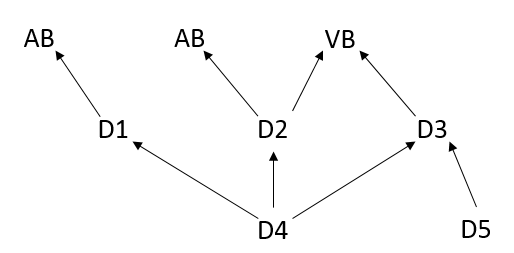
\includegraphics[scale=0.3]{grafik/classH}
\caption{Overview of the class hierarchy}
\label{classHierarchy}
\end{figure}

\subsubsection{The Class: VB}
By looking at the class hierarchy, we can see that VB is a virtual base class. A virtual base class, described in the C++ Book on page 631\cite{CplusplusBook}, is a class which is declared a virtual class by the classes that inherits it.
In code this is done in the Header file by writing the keyword virtual before the class, as showed in Listing \ref{virtualClass}.
\begin{lstlisting}[caption=Declaring a class virtual, label=virtualClass]
class D2 :
	public virtual VB, public AB
	{
	//Header file 
	}
	
class D3 :
	public virtual VB
	{
	//Header file 
	}
\end{lstlisting}
This declaration of a common virtual base enables the two classes to work on a shared copy of VB.
In order for them to do so the classes must both be inherited by the same class, creating a diamond like structure, in our case this is formed by VB, D2, D3 and D4 as shown in Figure\ref{diamondStructure}.
\begin{figure}[H]  
\centering
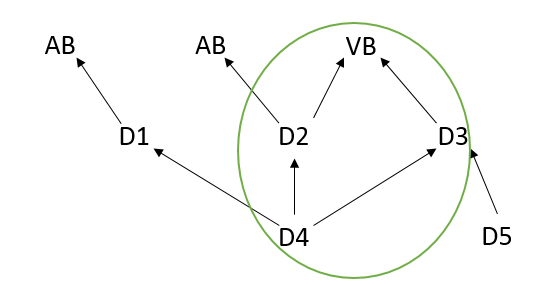
\includegraphics[scale=0.3]{grafik/diamondstructure}
\caption{Diamond structure marked by the green ring}
\label{diamondStructure}
\end{figure}
This diamond structure opens up for ambiguities between D2 and D3, which will be discuss later in section \ref{d4}.

\subsubsection{The Class: AB}
To finish the base classes move on to the class AB. AB is an abstract class, which means it should not be instantiatable. 
An abstract class, in C++, means that the class contains atleast one pure virtual function.
A pure virtual function, is a function which has been declare to be pure virtual meaning that is not implemented but instead have a pseudo initializer given by ''= 0''.
This is done as following, \lstinline$virtual void Incrementer() = 0;$, in the header file.
The AB class is furthermore designed to be a replicated base class. 
This means, unlike VB, that the class is replicated and two copies of AB class exist in our class hierarchy, as illustrated in Figure \ref{classHierarchy}.

\subsubsection{The Class: D1}
D1 is a class which simply overrides the pure virtual function in AB, which makes D1 instantiable. However this must be done properly since, as seen in the D1.h file line 15, hiding can also make the class instantiable and often result in undesired results.

\subsubsection{The Class: D2}
As the class hierarchy shows D2 inherits both from AB and virtual inherits from VB.
For D2 we add a new function \lstinline$ModifyRow$ which increments a row in the array from VB.
Furthermore it overrides the \lstinline$Incrementer$ function from AB and \lstinline$GetCombinedString$ from VB.

\subsubsection{The Class: D3}
This class virtual inherits from VB, and override the \lstinline$GetCombinedStrings$ function. This is setting the stage for an ambiguity, which will be discuss later in the report.

\subsubsection{The Class: D4}\label{d4}
As the class hierarchy shows this class inherits the most classes, which makes it the most complex and interesting one.\\
The class itself has two constructors \lstinline$D4(int, int, string);$ and a default one.
The interesting thing here is the appearance of the diamond structure mentioned earlier. 
The problem, mentioned in the C++ book on page 633, is that D4 should initialize D2 and D3 but both D2's and D3's constructor specifies the initializing of VB, and since VB is a shared copy by D2 and D3, it raises a question. 
What is the behaviour?
Should D2 go first and initialize the variables in VB and then get overriden by the initialization from D3? or the other way?
The answer is there should be no ambiguousness therefore is must be ensured that the virtual base constructor is only called exactly once, as mentioned in the C++ book page 633. 
Therefore, as seen in D4.cpp line 23, the compiler will translate the constructor seen in Listing \ref{NoGoodD4Constructor} to have an implicit initialization of the default constructor in VB.
But since VB does not have a default constructor the D4 constuctor shown in Listing \ref{NoGoodD4Constructor} is invalid.
\begin{lstlisting}[caption=Code snippet from D4.cpp file line 23, label=NoGoodD4Constructor]
D4::D4(int d1, int d2, string d3) : D3(d3 + "ThroughD4"), D1(d1), D2(d2)
{
	Couter<D4>().CoutType();
}
\end{lstlisting}
Therefore an explicit initialization of VB must be created, as shown in Listing \ref{D4explicitCallVB}, or a default constructor for VB necessary.
\begin{lstlisting}[caption=Code snippet from D4.cpp file line 5, label=D4explicitCallVB]
D4::D4(int d1, int d2, string d3) : D1(d1), D2(d2), D3(d3 + "ThroughD4"), VB(d3)
{
	cout << "Input - ";
	Couter<D4>().CoutType();
}
\end{lstlisting}
Here is a case regarding multiple inheritance which I find kinda dangerous, the implicit initialization of the default constructor of VB, makes the code hard to see through and, in my believe, has potential to cause serious issues. As illustrated in the D4 constructor, D3 gets a string for initialization, but the sole purpose is pass this string on to VB, this is exactly not good coding but it could happen.
The constructor now contains a parameter which is never being used or spoken off because of the implicit initialization. 
However this can of course be avoid by keep track of the fact that the virtual base constructor is called exactly once, but if the class hierarchy gets very complex it can be hard.\\\\
Moving on in the D4 Class we have a familiar function \lstinline$GetCombinedStrings()$ this overriding of the function is necessary because otherwise the functions from D2 and D3 would be ambiguous.
These functions is however not lost due to the override, but can still be called within D4, same goes for VB's functions, as shown in Listing \ref{getCombinedStringsD4}.
\begin{lstlisting}[caption=Code snippet from D4.cpp line 52, label=getCombinedStringsD4]
string D4::GetCombinedStrings()
{
	return "\nVB String: " + VB::GetCombinedStrings()
		+ "\nD2 String: " + D2::GetCombinedStrings() 
		+ "\nD3 String: " + D3::GetCombinedStrings();
}
\end{lstlisting}
The ''modify'' functions in D4 just shows that you can do modifications to the array both by using functions found inherited from D3 and D2, or by modifying directly on the array, given it is public or proctected as in C\# or Java.

\subsubsection{The Class: D5}\label{D5}
D5 is an almost empty class with a default constructor which will be used to test how a virtual inheritance behave with only one inherit.

\subsection{Tests}
There will be 4 test to verify/clarify different cases.
All the tests will be available in the Main.cpp file and marked with ''/*Test x: topic*/''.
\subsubsection{Test 1: Abstract instantiate and hiding}
The purpose of this test is to see what is possible when playing with abstract classes.
The results shows, as expected, that it is not possible to instantiate an abstract class due to the pure virtual function.

\subsubsection{Test 2: Replication and Upcasting}
The purpose of this test was to see the replicated AB classes in action.
Therefore the \lstinline$Incrementer()$ was modifed to increment D1 copy of AB by one and D2 copy of AB by two.
As result we got D4 is able to working on both copies of AB by going through D1 and D2, and by upcasting D4 to D1 we get the expected instance of AB.
However if we remake AB to be an not abstract class, and try to upcast D4 to AB it shows that this is not possible. 
This is due to the fact that there exist two instances of AB and it would be ambiguous.

\subsubsection{Test 3: Virtual Base}
The purpose of this test is to see virtual base in action.
To do so, D4 calls respectively the function which is inherited from D2 \lstinline$void ModifyRow(int);$ with 5 as parameter and the function which is inherited from D3 \lstinline$void ModifyColumn(int);$ with 3 as parameter.
Furthermore two custom function from D4 is called, \lstinline$void ModifyPoint(int, int);$ with parameter 5 and 3 and \lstinline$void ModifyRowAndColumn(int, int);$ with 10 and 10 as parameter.
The expected result from this, after the four calls, when we call the \lstinline$PrintMatrix$ function is that the array will contain a cross of 2's going through (3,5), (3,5) would be a 4 and (10,10) should be a 1.
The results were as expected and can be seen in Figure \ref{test3}.
\begin{figure}[H]  
\centering
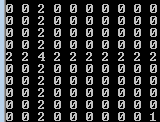
\includegraphics[scale=0.8]{grafik/resultTest3}
\caption{Result from Test 3}
\label{test3}
\end{figure}

\subsubsection{Test 4: What if there is only 1 inherit to a virtual base class}
This test, as described in Section \ref{D5} will be used to test how a virtual inheritance behave with only one inherit, as shown in Figure \ref{test5}.
\begin{figure}[H]  
\centering
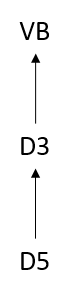
\includegraphics[scale=0.3]{grafik/test5}
\caption{Test 5 structure}
\label{test5}
\end{figure}
The result shows that even though D5 only inherits D3 and thus VB would only be constructed once by D3, the default constructor is still invoked in VB.
This of course streamlines the finding from Section \ref{d4}. 
But personally find it annoying that the implicit initializing through the default constructor happens, when I know the structure of the class diagram, and is able to see that i could use the other constructor.
So as a code convention I would suggest an explicit invoking of one of the VB constructors, as seen in Listing \ref{d5betterconstuctor}, to avoid unnecessary confusion.
\begin{lstlisting}[caption=Code snippet from D5.cpp line 10, label=d5betterconstuctor]
D5::D5() : D3("Used for nothing"), VB()
{
	Couter<D5>().CoutType();
}
\end{lstlisting}

\subsection{Reflection}
In general I find \textit{Multiple Inheritance} to be a great tool which, as mentioned in the C++ Book on page 624, leads to less code and more uniform code. 
Even though it has some dangerous pitfalls they seem to be manageable, and I find this to be true as long as you are careful with the complexity of the code.
Of course there is also the cases where you work on classes which is not created by yourself, thus making \textit{Multiple Inheritance} even more tricky.

Personally I liked the virtual based concept because this gives an easy entrance to working on a common object, like our array, without passing around the object or creating and managing the pointers yourself.
All in all I see great potential in \textit{Multiple Inheritance} if used with care. 
But also can I see the reasoning why languages like C\# and Java does not contain multiple inheritance for multiple reason.\\
Multiple inheritance does not give the language any more ''power'' and it can decrease readability. When working with virtual base classes you have to concentrate and make sure all the classes keep certain standard when working with the shared object and there is probably more which I have not yet discovered.
